%=========================================================================
% (c) Michal Bidlo, Bohuslav Křena, 2008

% Zajimavy blog
% http://brendangregg.com/

\chapter{Introduction}
Good application performance is one of the main goals during software development. Why is software performance so important? Bad software performance could have very unpleasant behavior not only for users, but also for application owner. Software reliability is guaranteed by owner, but with undesirable performance there could be a lot of issues which can badly influence software behavior hence this could lead to an outflow of the consumers, brand destruction, financial damage and loss of trust to the software owner. This few reasons are enough to do a proper performance testing before software release, which is more significant for many of large projects where large industries guarantee some level of software behavior and they cannot assure it after insufficient performance testing. Great emphasis on software performance is for example in space programs, medical facility, army systems or energy distribution systems. In such cases it is necessary to ensure proper application behavior for a long time with high load and without unsuspected behavior like as high response, frequent delay or stuck, because every failure could cost human lives. 

Nowadays every developer should trying to use frameworks which can make developers work easier because they can handle complex underlying issues such as security, performance and code clarity. It causes that developers can spend more time for the application functionality and meet the application requirements, because frameworks are usually optimized for particular job. In the past every developer had to spent more time with performance which lead to spent more time and money for software development, but not everyone have enough knowledge about performance testing and thus make performance analysis and optimization more difficult. This leads to need a special outsource performance tools which can provide more sophistic information however this tools are usually more expensive.

A very important part of performance analysis is the wise choice of \emph{key performance indicators} (KPIs) \cite{Molyneaux:TAoAPT} and clearly interpretation of the results as fast as possible. This can leads to faster detection of performance problems and help developers to fix them and meet the \emph{performance standards} \cite{Molyneaux:TAoAPT} set up by application owner or customer in time before the release cycle. 

In general an application performance is very important however network application or hardware performance is much more important nowadays when most communication is via internet.  When you make some payment in your internet banking you definitely want to have stable connection to your bank website without any delay. Network components like routers and switches are taken care of by the network stability hence it is very important to care about performance of those components. Network performance testing refers to measures of service quality of a network. When you want to buy some network hardware you probably want to know basic attributes such as \emph{bandwidth, throughput, latency} it has. During performance testing of network devices these, and more other attributes, are testing and evaluating. 

For performance testing of messaging system developed by \emph{Red Hat Inc.} there is the Messaging Performance Tool (MPT) \cite{ORPISKE:MSGPT}. MPT is intended for performance testing of \emph{Broker} \cite{RH:Broker} which is network application level software cooperating with \emph{Qpid-dispatch} \cite{RH:Interconnect} in the network as message distributor. Unfortunately, this tool does not have module for cover performance testing of Router component, Qpid-dispatch. 

This thesis describe fundamentals of performance testing which includes 'what is performance process', 'common performance issues', 'types of performance testing', 'standard performance metrics and how to choose them' and more in chapter \ref{Fundamentals of Software Performance Testing}. The rest of thesis is focused on performance testing and analysis of Qpid-dispatch, an application level router which is designed by Red Hat Inc. Qpid-dispatch performance testing is based on MPT which is described in chapter \ref{Messaging Performance Tool}. Description includes \emph{measures process} and \emph{gathered data description and evaluation}. Main goal is analyze MPT and design module for Qpid-dispatch performance testing. This part can be found in chapter \ref{Analysis and Design} just like a protocols which router working with and \emph{Automatic Topology Generator} for semi-automated network generating and deployment. After appropriate design, the implementation is needed, all used technologies, tools and  implementation processes of each component are described in chapter \ref{Implementation}. The most important part of the thesis is situated in chapter \ref{Experimental Evaluation}. It contains gathering data from routers located in different types of topology, their evaluation and representation which lead to conclusion about performance of Qpid-dispatch. Finally, chapter \ref{Conclusion} summarizes the thesis with our conclusion  and ideas for future use of developed tool.

% https://www.seguetech.com/what-is-software-performance-testing/

\chapter{Fundamentals of Software Performance Testing}
\label{Fundamentals of Software Performance Testing}
Main goal of performance testing is to ensure that an application runs fast enough to keep the attention of users, even with unexpected number of users using an application at the same time. Why is so important to have application optimized for best speed? It is simply, you are probably not only one person on the whole world with some application and when your application have slow response, long load time or bad scalability, the first website which user visit will be web of your competitor. That is the reason why speed is one of the most significant performance factor of common performance problems. This chapter summarize fundamentals of performance testing which includes common performance processes, issues and metrics. This chapter is based on knowledge available in \cite{Molyneaux:TAoAPT, Kurkova:Thesis:2017, DIN:PHD}.


\section{Performance Testing Process}
\label{Performance Testing Process}
Main goal of performance testing is to ensure following application attributes \cite{GAO:MEASURING}:

\begin{itemize}
	\setlength\itemsep{0em}
	\item \textbf{Reliability, Stability} \,---\ the ability of software to perform its functions in system environment under some system load for acceptable period of time
	\item \textbf{Scalability} \,---\ the ability of software to behave properly under various type of system load and handle growing up amount of work (network traffic, server load, data transfer)
	\item \textbf{Processing time, Speed} \,---\ the ability of software to react quickly without low response time during any acceptable system load
	\item \textbf{Availability} \,---\ the ability of software has available its functions during any acceptable system load
\end{itemize}

Performance testing process, as well as software development process, consist of all engineering steps from requirements definition to data evaluation. Between these steps is also found design, implementation of performance tests and execution with data gathering. 
\\

First step of performance testing process is selection of \emph{performance requirements} for the application. In this step, testing engineer has to analyze tested application, describe metrics, which will characterize an application performance and set performance requirements. It is very helpful to get answers for some questions about application:

\begin{itemize}
	\setlength\itemsep{0em}
	\item How many end users will the application need to support at release, after 6 months and 1 year ?
	\item Where will these users be located, and how will they connect to the application?
	\item How many end users will be concurrent at release, after 6 months and 1 year?
\end{itemize}

After complete this questions, an engineer should be able to select some important key performance indicators for performance test cases. Some of these indicators may be \emph{response time}, \emph{stability}, \emph{scalability} and \emph{speed}. However there are many other possible indicator so it is necessary to analyze whole application and take into consideration another application needs like error rate, system resources etc.  



\emph{workload} 

workload of testing environment

\todo{Dopsat kapitolu}

Graphical representation of the performance testing process is available on the figure~\ref{fig:performace_testing_process}. 

\begin{figure}[H]
  \centering
  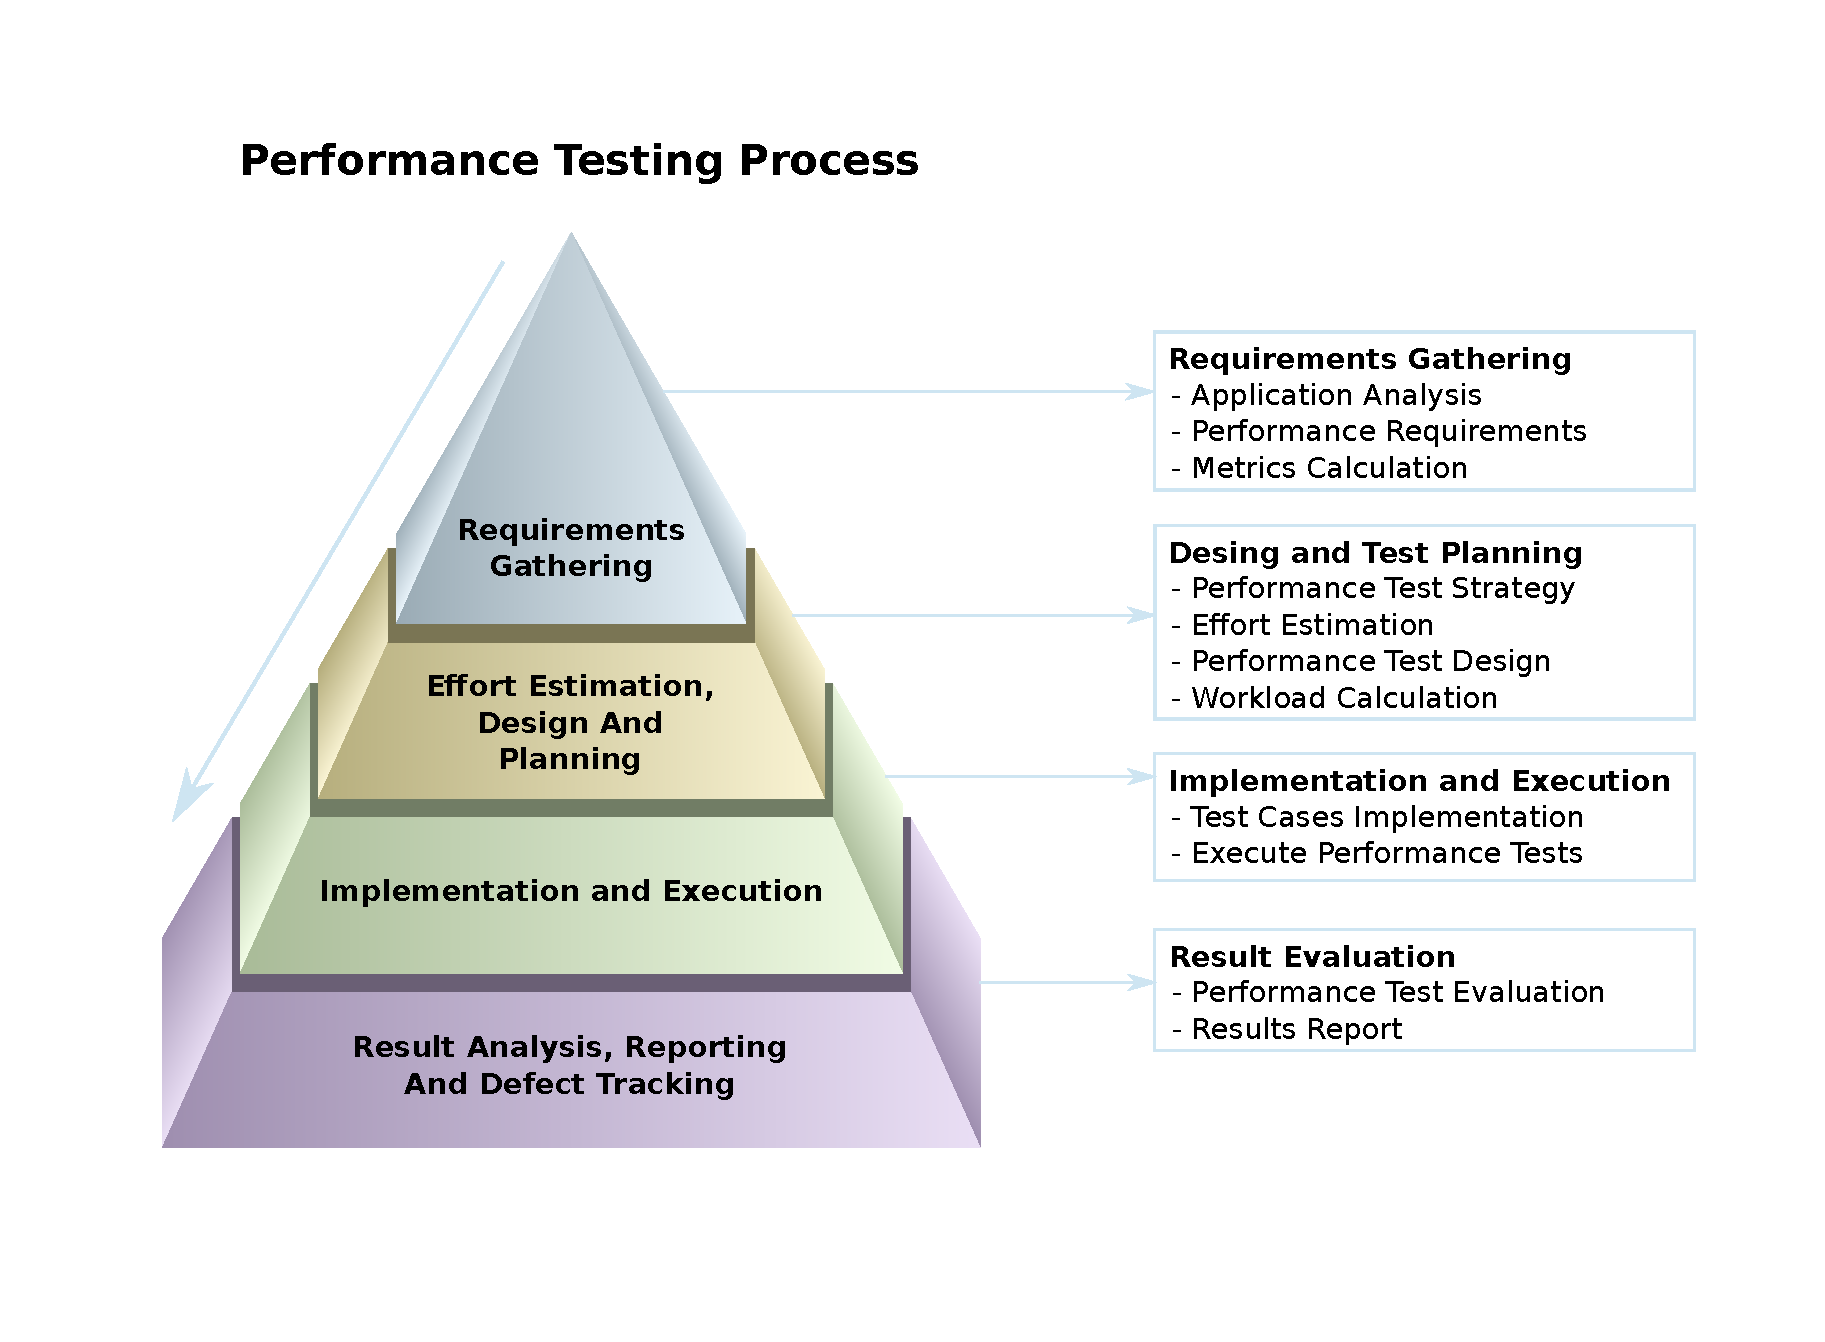
\includegraphics[width=16cm]{obrazky-figures/pyramid.pdf}
  \caption{Pyramid scheme of Performance Testing Process}
  \label{fig:performace_testing_process}
\end{figure}

\section{Performance Issues}
\label{Performance Issues}

\subsection{Response Time}

\subsection{Traffic Spikes}

\subsection{Performance Degradation}

\section{Different Types of Performance Testing}
\label{Different Types of Performance Testing}
% % http://www.wmrichards.com/high_performance_messaging.pdf 2017/10/18

\subsection*{Robustness Testing}
% Soak

\subsection*{Stress Testing}

\subsection*{Load Testing}

\subsection*{Bench-marking}

\section{Performance Metrics}
\label{Performance Metrics}
% https://loadstorm.com/load-testing-metrics/ 2017/10/18

\subsection{Response Time}

\subsection{Requests per Second}

\subsection{Resource Usage}

\subsection{Throughput}

\subsection{Error Rate}

\chapter{Messaging Performance Tool}
\label{Messaging Performance Tool}
% https://github.com/orpiske/msg-perf-tool

\section{Measures Process}
\label{Measures Process}

\section{Testing Metrics}
\label{Testing Metrics}

\section{Gathered Data and Their Evaluation}
\label{Gathered Data and Their Evaluation}

\section{Related Works}
\label{Related Works}
% popsat podobne "existujici" reseni (samozrejme, obcas neexistuje ;), ale verim, ze zde se neco najde). Nejlepsi je i se vuci tem "related tools" vymezit (jako napr. "The tool ... cannot be used because it does not support ...")

\chapter{Analysis and Design}
\label{Analysis and Design}

\section{Qpid-Dispatch Router}

\section{Usable Protocols}
AMQP, MQTT - possibly?

\section{Automatic Topology Generator}

\subsection{Network Components}

\subsection{Structure of Input and Output}

\subsection{Topology Creation}

\section{Qpid-Dispatch Performance Module}

\subsection{TODO - more subsections about module}

\section{Performance and Testing Metrics of Qpid-Dispatch Performance Module}

\section{Gathered Data Evaluation}

\chapter{Implementation}
\label{Implementation}

\section{Used Technologies}

\subsection{Ansible}

\subsection{Docker}
Using for testing Ansible roles (remove?)

\section{Topology Generator}

\subsection{Template Generator}

\subsection{Generation of Variables}

\subsection{Configuration Files Generation and Deployment}

\section{Qpid-Dispatch Performance Module}

\subsection{TODO - more subsections about implementation}

\chapter{Experimental Evaluation}
\label{Experimental Evaluation}

\section{Performance Testing on Various Generated Topology}

\section{Testing results}

\chapter{Conclusion}
\label{Conclusion}
%=========================================================================
